(\textit{Exercise 5.4 S\&B}) The pseudocode for \textit{Monte Carlo ES} is 
inefficient because, for each state-action pair, it maintains a list of all 
returns and repeatedly calculates their mean. How can we modify the algorithm
to have incremental updates for each state-action pair?
\begin{figure}[h!]
  \center
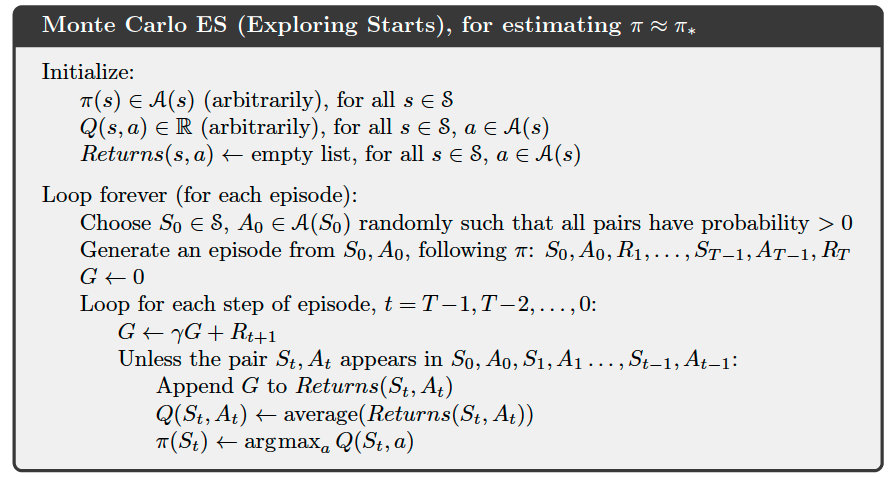
\includegraphics[width=0.8\linewidth]{figures/mc_es_pseudocode.png}
\end{figure}